% Options for packages loaded elsewhere
\PassOptionsToPackage{unicode}{hyperref}
\PassOptionsToPackage{hyphens}{url}
%
\documentclass[
]{article}
\usepackage{amsmath,amssymb}
\usepackage{lmodern}
\usepackage{iftex}
\ifPDFTeX
  \usepackage[T1]{fontenc}
  \usepackage[utf8]{inputenc}
  \usepackage{textcomp} % provide euro and other symbols
\else % if luatex or xetex
  \usepackage{unicode-math}
  \defaultfontfeatures{Scale=MatchLowercase}
  \defaultfontfeatures[\rmfamily]{Ligatures=TeX,Scale=1}
\fi
% Use upquote if available, for straight quotes in verbatim environments
\IfFileExists{upquote.sty}{\usepackage{upquote}}{}
\IfFileExists{microtype.sty}{% use microtype if available
  \usepackage[]{microtype}
  \UseMicrotypeSet[protrusion]{basicmath} % disable protrusion for tt fonts
}{}
\makeatletter
\@ifundefined{KOMAClassName}{% if non-KOMA class
  \IfFileExists{parskip.sty}{%
    \usepackage{parskip}
  }{% else
    \setlength{\parindent}{0pt}
    \setlength{\parskip}{6pt plus 2pt minus 1pt}}
}{% if KOMA class
  \KOMAoptions{parskip=half}}
\makeatother
\usepackage{xcolor}
\usepackage[margin=1in]{geometry}
\usepackage{color}
\usepackage{fancyvrb}
\newcommand{\VerbBar}{|}
\newcommand{\VERB}{\Verb[commandchars=\\\{\}]}
\DefineVerbatimEnvironment{Highlighting}{Verbatim}{commandchars=\\\{\}}
% Add ',fontsize=\small' for more characters per line
\usepackage{framed}
\definecolor{shadecolor}{RGB}{248,248,248}
\newenvironment{Shaded}{\begin{snugshade}}{\end{snugshade}}
\newcommand{\AlertTok}[1]{\textcolor[rgb]{0.94,0.16,0.16}{#1}}
\newcommand{\AnnotationTok}[1]{\textcolor[rgb]{0.56,0.35,0.01}{\textbf{\textit{#1}}}}
\newcommand{\AttributeTok}[1]{\textcolor[rgb]{0.77,0.63,0.00}{#1}}
\newcommand{\BaseNTok}[1]{\textcolor[rgb]{0.00,0.00,0.81}{#1}}
\newcommand{\BuiltInTok}[1]{#1}
\newcommand{\CharTok}[1]{\textcolor[rgb]{0.31,0.60,0.02}{#1}}
\newcommand{\CommentTok}[1]{\textcolor[rgb]{0.56,0.35,0.01}{\textit{#1}}}
\newcommand{\CommentVarTok}[1]{\textcolor[rgb]{0.56,0.35,0.01}{\textbf{\textit{#1}}}}
\newcommand{\ConstantTok}[1]{\textcolor[rgb]{0.00,0.00,0.00}{#1}}
\newcommand{\ControlFlowTok}[1]{\textcolor[rgb]{0.13,0.29,0.53}{\textbf{#1}}}
\newcommand{\DataTypeTok}[1]{\textcolor[rgb]{0.13,0.29,0.53}{#1}}
\newcommand{\DecValTok}[1]{\textcolor[rgb]{0.00,0.00,0.81}{#1}}
\newcommand{\DocumentationTok}[1]{\textcolor[rgb]{0.56,0.35,0.01}{\textbf{\textit{#1}}}}
\newcommand{\ErrorTok}[1]{\textcolor[rgb]{0.64,0.00,0.00}{\textbf{#1}}}
\newcommand{\ExtensionTok}[1]{#1}
\newcommand{\FloatTok}[1]{\textcolor[rgb]{0.00,0.00,0.81}{#1}}
\newcommand{\FunctionTok}[1]{\textcolor[rgb]{0.00,0.00,0.00}{#1}}
\newcommand{\ImportTok}[1]{#1}
\newcommand{\InformationTok}[1]{\textcolor[rgb]{0.56,0.35,0.01}{\textbf{\textit{#1}}}}
\newcommand{\KeywordTok}[1]{\textcolor[rgb]{0.13,0.29,0.53}{\textbf{#1}}}
\newcommand{\NormalTok}[1]{#1}
\newcommand{\OperatorTok}[1]{\textcolor[rgb]{0.81,0.36,0.00}{\textbf{#1}}}
\newcommand{\OtherTok}[1]{\textcolor[rgb]{0.56,0.35,0.01}{#1}}
\newcommand{\PreprocessorTok}[1]{\textcolor[rgb]{0.56,0.35,0.01}{\textit{#1}}}
\newcommand{\RegionMarkerTok}[1]{#1}
\newcommand{\SpecialCharTok}[1]{\textcolor[rgb]{0.00,0.00,0.00}{#1}}
\newcommand{\SpecialStringTok}[1]{\textcolor[rgb]{0.31,0.60,0.02}{#1}}
\newcommand{\StringTok}[1]{\textcolor[rgb]{0.31,0.60,0.02}{#1}}
\newcommand{\VariableTok}[1]{\textcolor[rgb]{0.00,0.00,0.00}{#1}}
\newcommand{\VerbatimStringTok}[1]{\textcolor[rgb]{0.31,0.60,0.02}{#1}}
\newcommand{\WarningTok}[1]{\textcolor[rgb]{0.56,0.35,0.01}{\textbf{\textit{#1}}}}
\usepackage{graphicx}
\makeatletter
\def\maxwidth{\ifdim\Gin@nat@width>\linewidth\linewidth\else\Gin@nat@width\fi}
\def\maxheight{\ifdim\Gin@nat@height>\textheight\textheight\else\Gin@nat@height\fi}
\makeatother
% Scale images if necessary, so that they will not overflow the page
% margins by default, and it is still possible to overwrite the defaults
% using explicit options in \includegraphics[width, height, ...]{}
\setkeys{Gin}{width=\maxwidth,height=\maxheight,keepaspectratio}
% Set default figure placement to htbp
\makeatletter
\def\fps@figure{htbp}
\makeatother
\setlength{\emergencystretch}{3em} % prevent overfull lines
\providecommand{\tightlist}{%
  \setlength{\itemsep}{0pt}\setlength{\parskip}{0pt}}
\setcounter{secnumdepth}{-\maxdimen} % remove section numbering
\ifLuaTeX
  \usepackage{selnolig}  % disable illegal ligatures
\fi
\IfFileExists{bookmark.sty}{\usepackage{bookmark}}{\usepackage{hyperref}}
\IfFileExists{xurl.sty}{\usepackage{xurl}}{} % add URL line breaks if available
\urlstyle{same} % disable monospaced font for URLs
\hypersetup{
  pdftitle={RDA trait prediction tutorial},
  pdfauthor={KE Lotterhos},
  hidelinks,
  pdfcreator={LaTeX via pandoc}}

\title{RDA trait prediction tutorial}
\author{KE Lotterhos}
\date{2023-02-08}

\begin{document}
\maketitle

This tutorial accompanies the paper ``The paradox of adaptive trait
clines with non-clinal patterns in the underlying genes'' published in
PNAS {[}add link{]}.

\hypertarget{abstract}{%
\section{Abstract}\label{abstract}}

Multivariate climate change presents an urgent need to understand how
species adapt to complex environments. Population genetic theory
predicts that loci under selection will form monotonic allele frequency
clines with their selective environment, which has led to the wide use
of genotype-environment associations (GEAs). However, the accuracy of
GEA methods to identify adapted loci is limited, as shown in the main
paper.

This tutorial shows how to apply a novel extension of multivariate
ordination, which accurately predicted individual multivariate traits
from genotype and environmental data on simulated data regardless of
whether inference from GEAs was accurate.

\hypertarget{install-packages}{%
\section{Install packages}\label{install-packages}}

If the following packages are not installed, be sure to install them
first:

\begin{verbatim}
install.packages("vegan")
install.packages("lfmm")
install.packages("gplots")

if (!require("BiocManager", quietly = TRUE))
    install.packages("BiocManager")

BiocManager::install("LEA")
\end{verbatim}

\hypertarget{load-the-libraries}{%
\subsection{Load the libraries:}\label{load-the-libraries}}

\begin{verbatim}
## Loading required package: permute
\end{verbatim}

\begin{verbatim}
## Loading required package: lattice
\end{verbatim}

\begin{verbatim}
## This is vegan 2.6-4
\end{verbatim}

\begin{verbatim}
## 
## Attaching package: 'LEA'
\end{verbatim}

\begin{verbatim}
## The following object is masked from 'package:lattice':
## 
##     barchart
\end{verbatim}

\begin{verbatim}
## 
## Attaching package: 'gplots'
\end{verbatim}

\begin{verbatim}
## The following object is masked from 'package:stats':
## 
##     lowess
\end{verbatim}

Don't forget to set your working directory!

\hypertarget{background-on-the-simulation}{%
\section{Background on the
simulation}\label{background-on-the-simulation}}

This data was simulated in SLiM and is associated with the complex
multivariate simulation presented in Figure 6 in the paper. Briefly, a
non-Wright-Fisher model was simulated on a landscape with 6
environmental variables that reflect different aspects of thermal stress
and precipitation in British Columbia. The simulation included 6
environmental traits, each of which adapted to a different environmental
variable.

The six environmental variables are based on real data from western
Canada and are shown below, clockwise from upper right: Clockwise from
upper left: precipitation of driest month, precipitation of warmest
quarter, mean annual temperature, precipitation of wettest month, mean
temperature of wettest quarter, mean temperature of driest quarter. Each
small square is a simulated individual, with its color representing its
trait value in that environment.

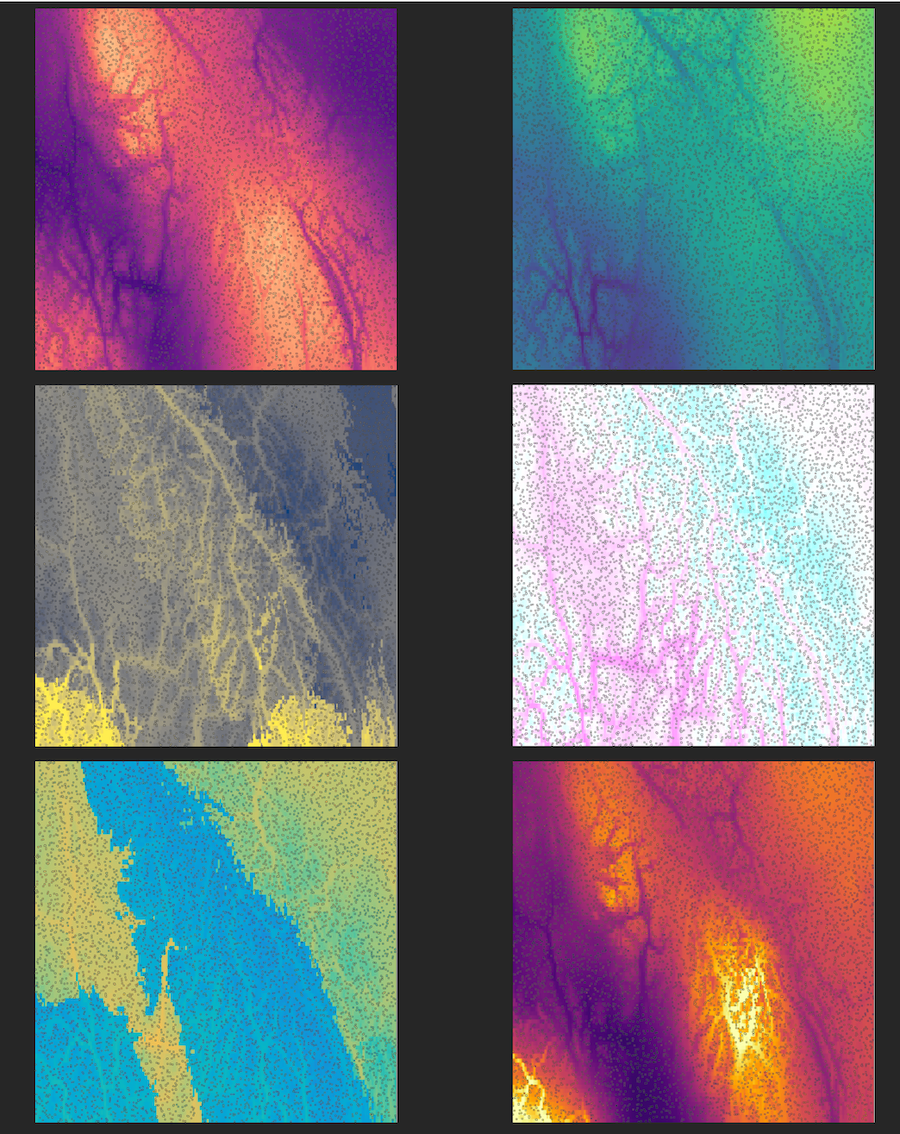
\includegraphics{multivar.png}

\hypertarget{load-the-data}{%
\section{Load the data}\label{load-the-data}}

\begin{itemize}
\tightlist
\item
  A matrix of genotypes in 012 format (counts of reference allele)

  \begin{itemize}
  \tightlist
  \item
    number of rows = number of individuals
  \item
    number of columns = number of SNPs
  \end{itemize}
\item
  A table with information about sampled individuals (each individual in
  a row)
\item
  A table with information about SNPs (each SNP in a row)
\end{itemize}

The \texttt{ind} table includes the xy location for each individual, the
6 exact trait values (note that these won't exactly equal the trait
value calculated from the genotype matrix because of MAF filtering), and
the 6 environmental values at their xy location.

The \texttt{muts} table includes the linkage group \texttt{LG}, the
position of the mutation on the genetic map \texttt{pos\_pyslim}, a
unique ID \texttt{mutname}, the allele frequency based on the 1000
sampled individuals \texttt{a\_freq\_subset}, and whether or not it had
effects on one or more phenotypes \texttt{causal}.

Note that you will have to change the working directory to where the
data is stored on your computer.

\begin{Shaded}
\begin{Highlighting}[]
\NormalTok{G }\OtherTok{\textless{}{-}} \FunctionTok{read.table}\NormalTok{(}\FunctionTok{unz}\NormalTok{(}\StringTok{"Genotypes.txt.zip"}\NormalTok{, }\StringTok{"Genotypes.txt"}\NormalTok{))}
\FunctionTok{dim}\NormalTok{(G) }\CommentTok{\# 1000 individuals and 26371 loci}
\end{Highlighting}
\end{Shaded}

\begin{verbatim}
## [1]  1000 26371
\end{verbatim}

\begin{Shaded}
\begin{Highlighting}[]
\NormalTok{ind }\OtherTok{\textless{}{-}} \FunctionTok{read.table}\NormalTok{(}\StringTok{"Individuals.txt"}\NormalTok{, }\AttributeTok{header=}\ConstantTok{TRUE}\NormalTok{)}
\FunctionTok{dim}\NormalTok{(ind) }\CommentTok{\#corresponds to rows in G}
\end{Highlighting}
\end{Shaded}

\begin{verbatim}
## [1] 1000   15
\end{verbatim}

\begin{Shaded}
\begin{Highlighting}[]
\FunctionTok{head}\NormalTok{(ind)}
\end{Highlighting}
\end{Shaded}

\begin{verbatim}
##   ind_index         x        y phenotype1_mat phenotype2_MTWetQ phenotype3_MTDQ
## 1        33 0.4061840 0.233272      0.7379670        -0.1914210        0.142992
## 2        34 0.4256970 0.837158     -0.2740810        -0.4283320       -0.012880
## 3        44 0.6716730 0.581744     -0.6763260         0.0866287       -0.470671
## 4        45 0.0174659 0.329922     -0.2832210        -0.4039420       -0.333718
## 5        46 0.0697436 0.121221      0.0576163        -0.3032010        0.731600
## 6        64 0.1433610 0.233237      0.2656280        -0.2318730        0.214004
##   phenotype4_PDM phenotype5_PwarmQ phenotype6_PWM  env1_mat env2_MTWetQ
## 1      -0.131894         -0.452497     -0.5416510  0.762432  -0.1622380
## 2       0.221058          0.229296      0.0665969 -0.339330  -0.4076670
## 3       0.218813          0.260098     -0.1034650 -0.567733   0.0909278
## 4      -0.200554         -0.345915     -0.4100010 -0.245860  -0.2007590
## 5       0.195679         -0.367110      0.1962960 -0.121500  -0.3063790
## 6      -0.239776         -0.517086     -0.2582660  0.103057  -0.2863170
##    env3_MTDQ  env4_PDM env5_PwarmQ   env6_PWM
## 1  0.2612810 -0.332078   -0.471502 -0.4778210
## 2 -0.0582962  0.288030    0.198810  0.0176800
## 3 -0.4143530  0.234899    0.230255 -0.0535109
## 4 -0.2674550 -0.265260   -0.389828 -0.4589790
## 5  0.7028580  0.211275   -0.352307  0.2127510
## 6  0.1657060 -0.190813   -0.476650 -0.2927740
\end{verbatim}

\begin{Shaded}
\begin{Highlighting}[]
\NormalTok{muts }\OtherTok{\textless{}{-}}  \FunctionTok{read.table}\NormalTok{(}\StringTok{"SNPs.txt"}\NormalTok{, }\AttributeTok{header=}\ConstantTok{TRUE}\NormalTok{)}
\FunctionTok{dim}\NormalTok{(muts) }\CommentTok{\#corresponds to columns in G}
\end{Highlighting}
\end{Shaded}

\begin{verbatim}
## [1] 26371     5
\end{verbatim}

\begin{Shaded}
\begin{Highlighting}[]
\FunctionTok{head}\NormalTok{(muts)}
\end{Highlighting}
\end{Shaded}

\begin{verbatim}
##   LG pos_pyslim mutname a_freq_subset causal
## 1  1          8     1-8        0.0175  FALSE
## 2  1         27    1-27        0.0120  FALSE
## 3  1         34    1-34        0.0370  FALSE
## 4  1         81    1-81        0.0330  FALSE
## 5  1         97    1-97        0.0170  FALSE
## 6  1        153   1-153        0.0225  FALSE
\end{verbatim}

\begin{Shaded}
\begin{Highlighting}[]
\FunctionTok{rownames}\NormalTok{(G) }\OtherTok{\textless{}{-}} \FunctionTok{as.character}\NormalTok{(}\FunctionTok{paste0}\NormalTok{(}\StringTok{"i\_"}\NormalTok{,ind}\SpecialCharTok{$}\NormalTok{ind\_index))}
\FunctionTok{colnames}\NormalTok{(G) }\OtherTok{\textless{}{-}} \FunctionTok{as.character}\NormalTok{(muts}\SpecialCharTok{$}\NormalTok{mutname)}
\CommentTok{\#G \textless{}{-} as.matrix(G)}
\FunctionTok{head}\NormalTok{(G[,}\DecValTok{1}\SpecialCharTok{:}\DecValTok{10}\NormalTok{])}
\end{Highlighting}
\end{Shaded}

\begin{verbatim}
##      1-8 1-27 1-34 1-81 1-97 1-153 1-154 1-206 1-287 1-304
## i_33   0    0    0    0    0     0     0     0     0     0
## i_34   0    0    0    0    0     0     0     0     0     0
## i_44   0    0    0    0    0     0     0     0     0     0
## i_45   0    0    0    0    0     0     0     0     0     0
## i_46   0    0    0    0    0     0     0     0     1     0
## i_64   2    0    0    0    0     0     0     0     0     0
\end{verbatim}

\hypertarget{rda-trait-prediction-function}{%
\section{RDA trait prediction
function}\label{rda-trait-prediction-function}}

This function predicts an environmental trait through the
back-transformation of the RDA ``site score'' of an individual to a
chosen environmental variable (Equation 1 in the manuscript). It makes
the prediction for all the individuals that were used to run the RDA.

\begin{Shaded}
\begin{Highlighting}[]
\NormalTok{rda\_trait\_pred }\OtherTok{\textless{}{-}} \ControlFlowTok{function}\NormalTok{(rdaobj, env\_row, K)\{}
  \CommentTok{\#rdaobj is RDA object}
  \CommentTok{\#env\_row is the row of the environment in the biplot output}
  \CommentTok{\#K is the number of RDA axes}
\NormalTok{  scores }\OtherTok{\textless{}{-}} \FunctionTok{scores}\NormalTok{(rdaobj, }\AttributeTok{choices=}\DecValTok{1}\SpecialCharTok{:}\NormalTok{K)}
\NormalTok{  ind.sc }\OtherTok{\textless{}{-}}\NormalTok{ scores}\SpecialCharTok{$}\NormalTok{sites}
\NormalTok{  pred }\OtherTok{\textless{}{-}} \FunctionTok{matrix}\NormalTok{(}\ConstantTok{NA}\NormalTok{, }\AttributeTok{nrow=}\FunctionTok{nrow}\NormalTok{(ind.sc), }\AttributeTok{ncol=}\NormalTok{K)}
  \ControlFlowTok{for}\NormalTok{ (k }\ControlFlowTok{in} \DecValTok{1}\SpecialCharTok{:}\NormalTok{K)\{}
\NormalTok{    pred[,k] }\OtherTok{\textless{}{-}}\NormalTok{ ind.sc[,k]}\SpecialCharTok{*}\FunctionTok{eigenvals}\NormalTok{(rdaobj)[k]}\SpecialCharTok{*}\FunctionTok{summary}\NormalTok{(rdaobj)}\SpecialCharTok{$}\NormalTok{biplot[env\_row,k]}
\NormalTok{  \}}
\NormalTok{  trait\_pred }\OtherTok{\textless{}{-}} \FunctionTok{scale}\NormalTok{(}\FunctionTok{rowSums}\NormalTok{(pred))}
 \FunctionTok{return}\NormalTok{(trait\_pred) }
\NormalTok{\}}
\end{Highlighting}
\end{Shaded}

\hypertarget{example-of-an-rda-predicted-environmental-trait-value}{%
\subsection{Example of an RDA-predicted environmental trait
value}\label{example-of-an-rda-predicted-environmental-trait-value}}

\begin{enumerate}
\def\labelenumi{\arabic{enumi}.}
\tightlist
\item
  First, run the RDA:
\end{enumerate}

Scale the environmental variables to have a mean of 0 and standard
deviation of 1.

\begin{Shaded}
\begin{Highlighting}[]
\NormalTok{ind}\SpecialCharTok{$}\NormalTok{env1\_mat }\OtherTok{\textless{}{-}} \FunctionTok{scale}\NormalTok{(ind}\SpecialCharTok{$}\NormalTok{env1\_mat)}
\NormalTok{ind}\SpecialCharTok{$}\NormalTok{env2\_MTWetQ }\OtherTok{\textless{}{-}} \FunctionTok{scale}\NormalTok{(ind}\SpecialCharTok{$}\NormalTok{env2\_MTWetQ)}
\NormalTok{ind}\SpecialCharTok{$}\NormalTok{env3\_MTDQ }\OtherTok{\textless{}{-}} \FunctionTok{scale}\NormalTok{(ind}\SpecialCharTok{$}\NormalTok{env3\_MTDQ)}
\NormalTok{ind}\SpecialCharTok{$}\NormalTok{env4\_PDM }\OtherTok{\textless{}{-}} \FunctionTok{scale}\NormalTok{(ind}\SpecialCharTok{$}\NormalTok{env4\_PDM)}
\NormalTok{ind}\SpecialCharTok{$}\NormalTok{env5\_PwarmQ }\OtherTok{\textless{}{-}} \FunctionTok{scale}\NormalTok{(ind}\SpecialCharTok{$}\NormalTok{env5\_PwarmQ)}
\NormalTok{ind}\SpecialCharTok{$}\NormalTok{env6\_PWM }\OtherTok{\textless{}{-}} \FunctionTok{scale}\NormalTok{(ind}\SpecialCharTok{$}\NormalTok{env6\_PWM)}

\CommentTok{\# Run the RDA}
\NormalTok{rdaout }\OtherTok{\textless{}{-}} \FunctionTok{rda}\NormalTok{(G }\SpecialCharTok{\textasciitilde{}}\NormalTok{ ind}\SpecialCharTok{$}\NormalTok{env1\_mat }\SpecialCharTok{+}
\NormalTok{                ind}\SpecialCharTok{$}\NormalTok{env2\_MTWetQ }\SpecialCharTok{+}
\NormalTok{                ind}\SpecialCharTok{$}\NormalTok{env3\_MTDQ }\SpecialCharTok{+} 
\NormalTok{                ind}\SpecialCharTok{$}\NormalTok{env4\_PDM }\SpecialCharTok{+}
\NormalTok{                ind}\SpecialCharTok{$}\NormalTok{env5\_PwarmQ }\SpecialCharTok{+}
\NormalTok{                ind}\SpecialCharTok{$}\NormalTok{env6\_PWM}
\NormalTok{              )}
\end{Highlighting}
\end{Shaded}

\begin{enumerate}
\def\labelenumi{\arabic{enumi}.}
\setcounter{enumi}{1}
\tightlist
\item
  Next, check the biplot output and decide how many RDA axes to use in
  the prediction.
\end{enumerate}

\begin{Shaded}
\begin{Highlighting}[]
\CommentTok{\# Check the biplot output}
\NormalTok{rdaout}\SpecialCharTok{$}\NormalTok{CCA}\SpecialCharTok{$}\NormalTok{biplot}
\end{Highlighting}
\end{Shaded}

\begin{verbatim}
##                       RDA1        RDA2       RDA3        RDA4        RDA5
## ind$env1_mat    -0.5004451  0.01863416 -0.5476147  0.54418964 -0.37298079
## ind$env2_MTWetQ  0.4523477  0.19158505 -0.8296969 -0.11392353  0.03132509
## ind$env3_MTDQ   -0.7128197 -0.22757653  0.1200761  0.48309488  0.33816827
## ind$env4_PDM    -0.3843437  0.04904761  0.8297919 -0.24744529  0.09707124
## ind$env5_PwarmQ  0.6524152  0.56221376  0.4505148  0.02427266 -0.04630498
## ind$env6_PWM     0.3209795 -0.05176393  0.7346369  0.19495732 -0.08780176
##                       RDA6
## ind$env1_mat    -0.1186113
## ind$env2_MTWetQ -0.2373183
## ind$env3_MTDQ   -0.2791780
## ind$env4_PDM    -0.3011107
## ind$env5_PwarmQ -0.2292885
## ind$env6_PWM    -0.5557731
\end{verbatim}

\begin{Shaded}
\begin{Highlighting}[]
\CommentTok{\# Decide how many RDA axes to use in calculation}
\NormalTok{  a}\OtherTok{\textless{}{-}} \FunctionTok{screeplot}\NormalTok{(rdaout)}
\end{Highlighting}
\end{Shaded}

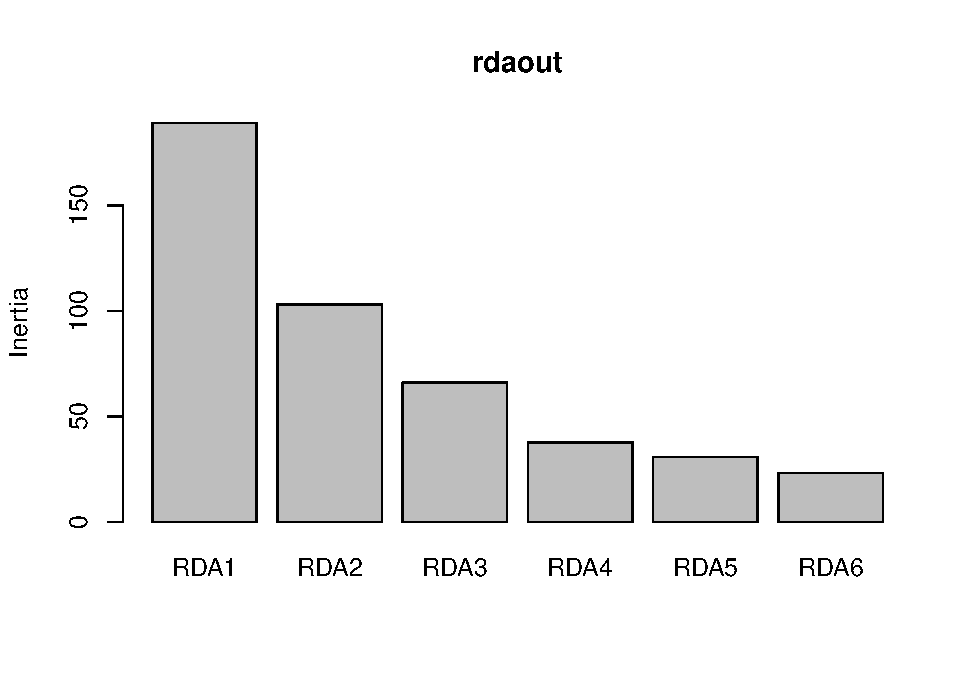
\includegraphics{RDAtraitPredictionTutorial_files/figure-latex/unnamed-chunk-1-1.pdf}

\begin{Shaded}
\begin{Highlighting}[]
  \FunctionTok{str}\NormalTok{(a)}
\end{Highlighting}
\end{Shaded}

\begin{verbatim}
## List of 4
##  $ x   : num [1:6] 0.7 1.9 3.1 4.3 5.5 6.7
##  $ y   : num [1:6] 189 103.1 66.1 37.8 30.9 ...
##  $ xlab: NULL
##  $ ylab: NULL
\end{verbatim}

\begin{Shaded}
\begin{Highlighting}[]
\NormalTok{  a}\SpecialCharTok{$}\NormalTok{y }\CommentTok{\# save this it\textquotesingle{}s the eigenvalues}
\end{Highlighting}
\end{Shaded}

\begin{verbatim}
## [1] 189.02481 103.10740  66.10749  37.79033  30.86247  23.24983
\end{verbatim}

\begin{Shaded}
\begin{Highlighting}[]
\NormalTok{  prop\_var }\OtherTok{\textless{}{-}} \FunctionTok{round}\NormalTok{(a}\SpecialCharTok{$}\NormalTok{y[}\DecValTok{1}\SpecialCharTok{:}\DecValTok{6}\NormalTok{]}\SpecialCharTok{/}\FunctionTok{sum}\NormalTok{(a}\SpecialCharTok{$}\NormalTok{y),}\DecValTok{3}\NormalTok{)}
  \FunctionTok{cumsum}\NormalTok{(prop\_var)}
\end{Highlighting}
\end{Shaded}

\begin{verbatim}
## [1] 0.420 0.649 0.796 0.880 0.949 1.001
\end{verbatim}

\begin{Shaded}
\begin{Highlighting}[]
  \FunctionTok{plot}\NormalTok{(}\FunctionTok{cumsum}\NormalTok{(prop\_var), }\AttributeTok{xlab=}\StringTok{"Number of RDA axes"}\NormalTok{, }
       \AttributeTok{ylab=}\StringTok{"Cumulative percent of variation explained"}\NormalTok{, }\AttributeTok{ylim=}\FunctionTok{c}\NormalTok{(}\DecValTok{0}\NormalTok{,}\DecValTok{1}\NormalTok{))}
\end{Highlighting}
\end{Shaded}

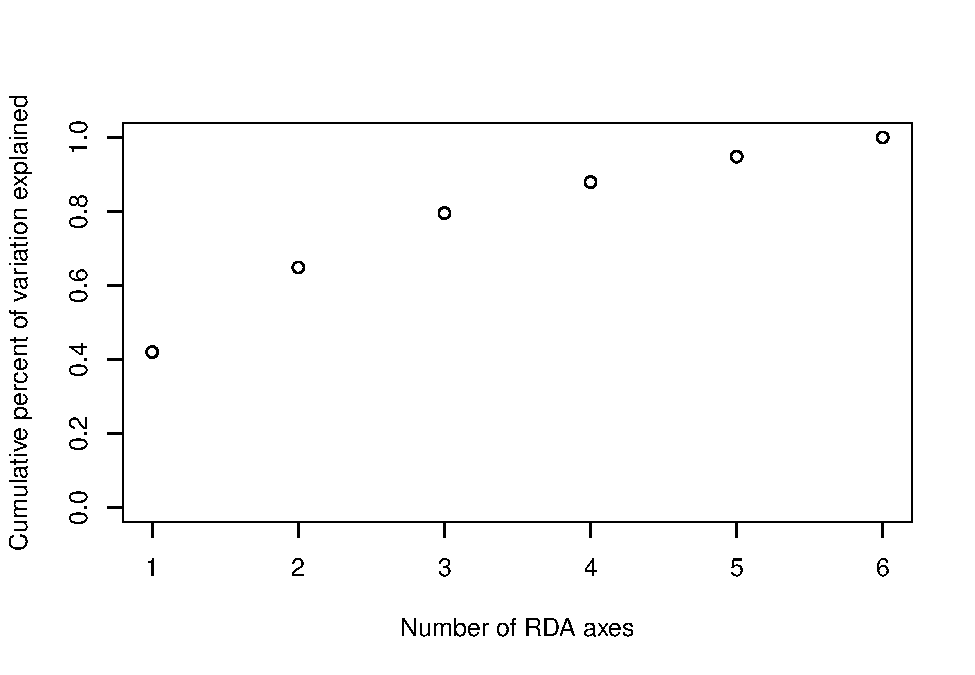
\includegraphics{RDAtraitPredictionTutorial_files/figure-latex/unnamed-chunk-1-2.pdf}

\begin{enumerate}
\def\labelenumi{\arabic{enumi}.}
\setcounter{enumi}{2}
\tightlist
\item
  In this case, the first 3 RDA axes explain 80\% of the variance. Note
  that choosing too many axes may result in overfitting. Here is an
  example of a trait prediction for MAT using the first 3 RDA axes:
\end{enumerate}

\begin{Shaded}
\begin{Highlighting}[]
\CommentTok{\# Make the trait prediction for MAT (1st row in biplot output)}
\NormalTok{K }\OtherTok{=} \DecValTok{3} \CommentTok{\# use 3 RDA axes to make the trait prediction}

\NormalTok{MATtraitPredict }\OtherTok{\textless{}{-}} \FunctionTok{rda\_trait\_pred}\NormalTok{(rdaout, }\DecValTok{1}\NormalTok{, K)}

\CommentTok{\# Since this is a simulation, we can compare the prediction to the true value}
\CommentTok{\# Similarly, an empirical study could compare an empirically measured trait value }
\CommentTok{\# to the RDA{-}predicted trait value to test how well landscape genomic data }
\CommentTok{\# can predict functional traits}
\FunctionTok{plot}\NormalTok{(}\FunctionTok{scale}\NormalTok{(ind}\SpecialCharTok{$}\NormalTok{phenotype1\_mat), MATtraitPredict, }\AttributeTok{xlab=}\StringTok{"Evolved trait value in simulations"}\NormalTok{,}
     \AttributeTok{ylab=}\StringTok{"RDA trait prediction"}\NormalTok{)}
\FunctionTok{abline}\NormalTok{(}\DecValTok{0}\NormalTok{,}\DecValTok{1}\NormalTok{)}
\end{Highlighting}
\end{Shaded}

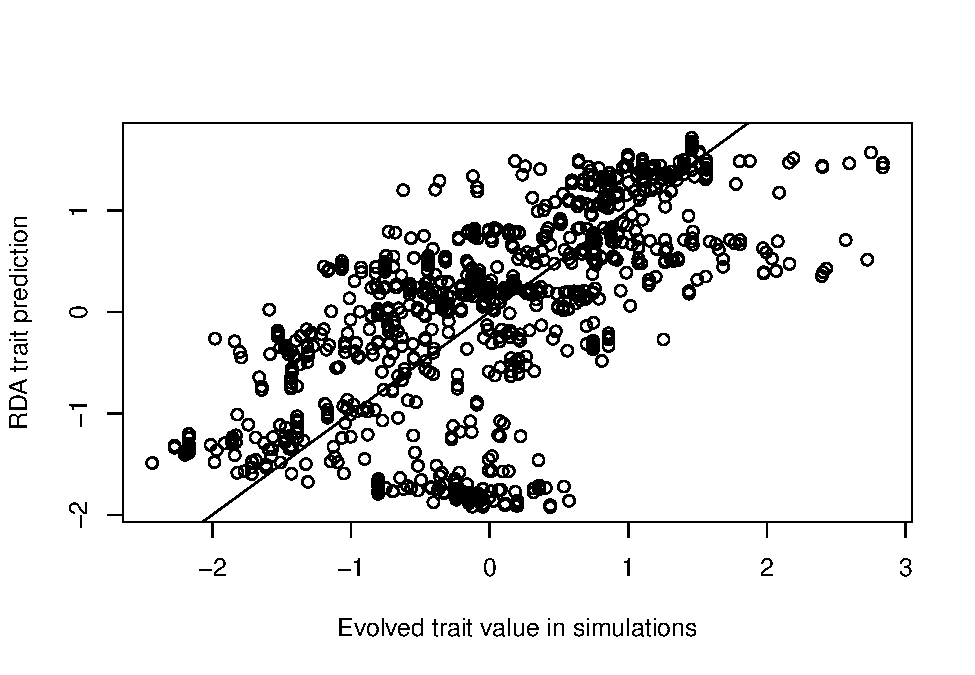
\includegraphics{RDAtraitPredictionTutorial_files/figure-latex/unnamed-chunk-2-1.pdf}

\begin{Shaded}
\begin{Highlighting}[]
\CommentTok{\#Correlation between the prediction and the true value:}
\FunctionTok{cor}\NormalTok{(ind}\SpecialCharTok{$}\NormalTok{phenotype1\_mat, MATtraitPredict) }
\end{Highlighting}
\end{Shaded}

\begin{verbatim}
##           [,1]
## [1,] 0.6461756
\end{verbatim}

\hypertarget{compare-to-other-functions-in-rda}{%
\subsubsection{Compare to other functions in
RDA}\label{compare-to-other-functions-in-rda}}

Note that the \texttt{predict} function and it's variations in the R
package \texttt{vegan} do not make the same kind of predictions as
\texttt{rda\_trait\_pred}. Here are the types of outputs produced by the
function \texttt{predict} and its variations:

\begin{Shaded}
\begin{Highlighting}[]
\CommentTok{\# This option in the \textasciigrave{}predict\textasciigrave{} function outputs the scores for each locus in RDA space}
\NormalTok{loci\_scores\_predict }\OtherTok{\textless{}{-}} \FunctionTok{predict}\NormalTok{(rdaout, }\AttributeTok{type=}\StringTok{"sp"}\NormalTok{, }\AttributeTok{newdata=}\NormalTok{G, }\AttributeTok{scaling=}\DecValTok{2}\NormalTok{)}
\FunctionTok{str}\NormalTok{(loci\_scores\_predict)}
\end{Highlighting}
\end{Shaded}

\begin{verbatim}
##  num [1:26371, 1:6] -0.00957 -0.01685 -0.00659 0.08155 0.03396 ...
##  - attr(*, "dimnames")=List of 2
##   ..$ : chr [1:26371] "1-8" "1-27" "1-34" "1-81" ...
##   ..$ : chr [1:6] "RDA1" "RDA2" "RDA3" "RDA4" ...
\end{verbatim}

\begin{Shaded}
\begin{Highlighting}[]
\CommentTok{\# This option in the \textasciigrave{}predict\textasciigrave{} function outputs the fitted values from the multiple regression}
\CommentTok{\# performed on each locus within each individual }
\NormalTok{fitted\_values\_predict }\OtherTok{\textless{}{-}} \FunctionTok{predict}\NormalTok{(rdaout, }\AttributeTok{newdata=}\NormalTok{G, }\AttributeTok{type=}\StringTok{"response"}\NormalTok{)}
\FunctionTok{str}\NormalTok{(fitted\_values\_predict)}
\end{Highlighting}
\end{Shaded}

\begin{verbatim}
##  num [1:1000, 1:26371] 0.1031 0.0345 -0.0436 0.1821 0.1753 ...
##  - attr(*, "dimnames")=List of 2
##   ..$ : chr [1:1000] "i_33" "i_34" "i_44" "i_45" ...
##   ..$ : chr [1:26371] "1-8" "1-27" "1-34" "1-81" ...
\end{verbatim}

\begin{Shaded}
\begin{Highlighting}[]
  \CommentTok{\# As a side note, it outputs the same thing as the \textasciigrave{}fitted\textasciigrave{} function}
\NormalTok{  fitted\_values\_predict2 }\OtherTok{\textless{}{-}} \FunctionTok{fitted}\NormalTok{(rdaout)}
  \FunctionTok{str}\NormalTok{(fitted\_values\_predict2)}
\end{Highlighting}
\end{Shaded}

\begin{verbatim}
##  num [1:1000, 1:26371] 0.1031 0.0345 -0.0436 0.1821 0.1753 ...
##  - attr(*, "METHOD")= chr "PCA"
##  - attr(*, "dimnames")=List of 2
##   ..$ : chr [1:1000] "i_33" "i_34" "i_44" "i_45" ...
##   ..$ : chr [1:26371] "1-8" "1-27" "1-34" "1-81" ...
\end{verbatim}

\begin{Shaded}
\begin{Highlighting}[]
\CommentTok{\# This option  in the \textasciigrave{}predict\textasciigrave{} function outputs the individual scores in RDA space }
\CommentTok{\# based on a linear combination of the predictor variables}
\NormalTok{X }\OtherTok{\textless{}{-}} \FunctionTok{data.frame}\NormalTok{(ind}\SpecialCharTok{$}\NormalTok{env1\_mat ,}
\NormalTok{                ind}\SpecialCharTok{$}\NormalTok{env2\_MTWetQ ,}
\NormalTok{                ind}\SpecialCharTok{$}\NormalTok{env3\_MTDQ ,}
\NormalTok{                ind}\SpecialCharTok{$}\NormalTok{env4\_PDM ,}
\NormalTok{                ind}\SpecialCharTok{$}\NormalTok{env5\_PwarmQ ,}
\NormalTok{                ind}\SpecialCharTok{$}\NormalTok{env6\_PWM)}
\NormalTok{ind\_scores\_predict }\OtherTok{\textless{}{-}} \FunctionTok{predict}\NormalTok{(rdaout, }\AttributeTok{type=}\StringTok{"lc"}\NormalTok{, }\AttributeTok{new=}\NormalTok{X, }\AttributeTok{scal=}\DecValTok{2}\NormalTok{)}
\FunctionTok{str}\NormalTok{(ind\_scores\_predict)}
\end{Highlighting}
\end{Shaded}

\begin{verbatim}
##  num [1:1000, 1:6] -2.034 -0.19 0.543 0.253 -0.508 ...
##  - attr(*, "dimnames")=List of 2
##   ..$ : chr [1:1000] "1" "2" "3" "4" ...
##   ..$ : chr [1:6] "RDA1" "RDA2" "RDA3" "RDA4" ...
\end{verbatim}

The \texttt{predict} function and its variations make predictions in RDA
space, and therefore do not output the same kind of predictions as
\texttt{rda\_trait\_predict} and Equation 1 in the paper.

\hypertarget{understanding-how-the-rda-is-built-on-multiple-regressions}{%
\section{Understanding how the RDA is built on multiple
regressions}\label{understanding-how-the-rda-is-built-on-multiple-regressions}}

Prior to ordination in the RDA, each locus is used in a multiple
regression model with the environmental variables to produce fitted
values for that locus across individuals.

\emph{SNP Genotype} \textasciitilde{} \emph{Env1} + \emph{Env2} +
\emph{Env3} etc.

For example for the first SNP in the data:

\begin{Shaded}
\begin{Highlighting}[]
 \CommentTok{\# multiple regression of 1st locus}

\NormalTok{mod }\OtherTok{\textless{}{-}} \FunctionTok{lm}\NormalTok{(G[,}\DecValTok{1}\NormalTok{] }\SpecialCharTok{\textasciitilde{}}\NormalTok{ ind}\SpecialCharTok{$}\NormalTok{env1\_mat }\SpecialCharTok{+}\NormalTok{ ind}\SpecialCharTok{$}\NormalTok{env2\_MTWetQ }\SpecialCharTok{+}\NormalTok{ ind}\SpecialCharTok{$}\NormalTok{env3\_MTDQ }\SpecialCharTok{+}\NormalTok{  ind}\SpecialCharTok{$}\NormalTok{env4\_PDM }\SpecialCharTok{+}
\NormalTok{                ind}\SpecialCharTok{$}\NormalTok{env5\_PwarmQ }\SpecialCharTok{+}\NormalTok{   ind}\SpecialCharTok{$}\NormalTok{env6\_PWM)}
 \FunctionTok{coef}\NormalTok{(}\FunctionTok{summary}\NormalTok{(mod))}
\end{Highlighting}
\end{Shaded}

\begin{verbatim}
##                     Estimate  Std. Error    t value     Pr(>|t|)
## (Intercept)      0.035000000 0.007404071  4.7271290 2.605782e-06
## ind$env1_mat    -0.035729076 0.011338501 -3.1511287 1.675100e-03
## ind$env2_MTWetQ -0.062538545 0.012165353 -5.1407094 3.295576e-07
## ind$env3_MTDQ    0.007471565 0.013224098  0.5649962 5.722040e-01
## ind$env4_PDM    -0.088670803 0.014835808 -5.9768099 3.169042e-09
## ind$env5_PwarmQ -0.069588746 0.014273932 -4.8752331 1.264746e-06
## ind$env6_PWM     0.047203246 0.013582893  3.4751982 5.325440e-04
\end{verbatim}

Although multiple regression is a linear combination of multiple
variables, it is able to model complex multivariate responses that
appear to be non-monotonic in any one dimension. For example, let's look
at a the relationship between explanatory variable temperature and the
response variable genotype, across decreasing and increasing values of
the other explanatory variables:

\begin{Shaded}
\begin{Highlighting}[]
\NormalTok{otherenv }\OtherTok{\textless{}{-}} \FunctionTok{c}\NormalTok{(}\FunctionTok{seq}\NormalTok{(}\DecValTok{1}\NormalTok{,}\DecValTok{0}\NormalTok{,}\AttributeTok{length.out=}\DecValTok{100}\NormalTok{), }\FunctionTok{seq}\NormalTok{(}\DecValTok{0}\NormalTok{,}\DecValTok{1}\NormalTok{,}\AttributeTok{length.out=}\DecValTok{101}\NormalTok{))}
\NormalTok{newdata}\OtherTok{=}\FunctionTok{data.frame}\NormalTok{(}\AttributeTok{ind.env1\_mat =} \FunctionTok{seq}\NormalTok{(}\SpecialCharTok{{-}}\DecValTok{1}\NormalTok{,}\DecValTok{1}\NormalTok{, }\AttributeTok{by=}\FloatTok{0.01}\NormalTok{),}
                   \AttributeTok{ind.env2\_MTWetQ =}\NormalTok{ otherenv,}
                   \AttributeTok{ind.env3\_MTDQ =}\NormalTok{ otherenv,}
                   \AttributeTok{ind.env4\_PDM =}\NormalTok{ otherenv,}
                   \AttributeTok{ind.env5\_PwarmQ =}\NormalTok{otherenv,}
                   \AttributeTok{ind.env6\_PWM =}\NormalTok{ otherenv)}
\NormalTok{pred }\OtherTok{\textless{}{-}} \FunctionTok{t}\NormalTok{(newdata)}\SpecialCharTok{*}\NormalTok{(}\FunctionTok{coef}\NormalTok{(}\FunctionTok{summary}\NormalTok{(mod))[}\DecValTok{2}\SpecialCharTok{:}\DecValTok{7}\NormalTok{,}\DecValTok{1}\NormalTok{]) }\SpecialCharTok{+} \FunctionTok{coef}\NormalTok{(}\FunctionTok{summary}\NormalTok{(mod))[}\DecValTok{1}\NormalTok{,}\DecValTok{1}\NormalTok{]}
\FunctionTok{plot}\NormalTok{(}\FunctionTok{seq}\NormalTok{(}\SpecialCharTok{{-}}\DecValTok{1}\NormalTok{,}\DecValTok{1}\NormalTok{, }\AttributeTok{by=}\FloatTok{0.01}\NormalTok{), }\FunctionTok{colSums}\NormalTok{(pred), }\AttributeTok{xlab=}\StringTok{"Temperature"}\NormalTok{, }\AttributeTok{ylab=}\StringTok{"Genotype prediction"}\NormalTok{)}
\end{Highlighting}
\end{Shaded}

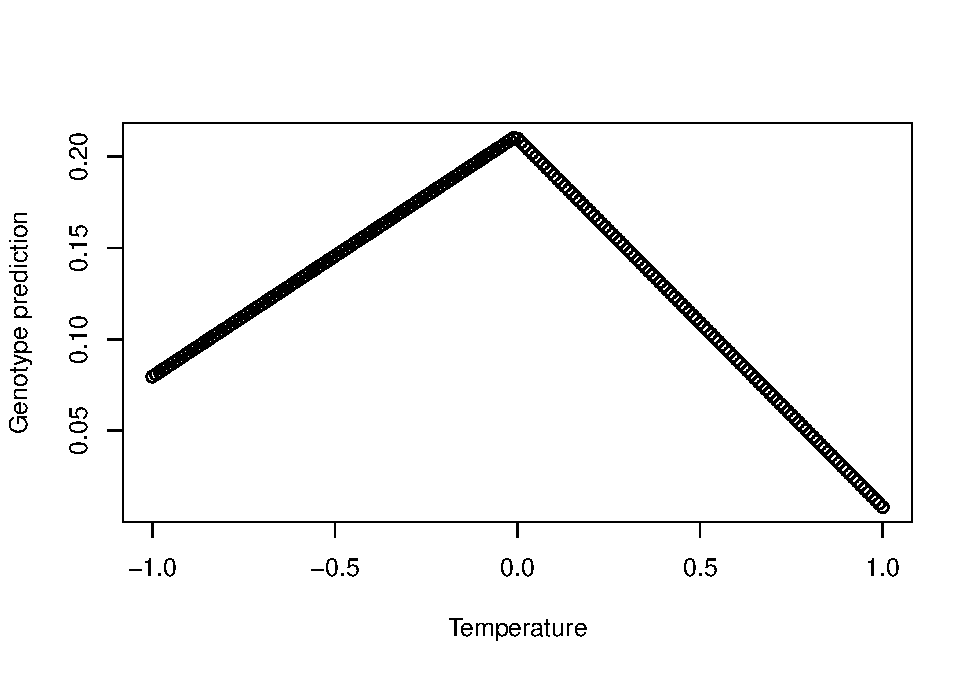
\includegraphics{RDAtraitPredictionTutorial_files/figure-latex/unnamed-chunk-5-1.pdf}

Thus, there is flexibility with the RDA to capture the way environmental
variables may influence the patterns at one locus in a different way
than at another locus, which may not correlate with the relationship
between the environment and population structure.

It may be interesting for some studies to understand how each locus is
shaped by the environment - in other words, what are the slopes
associated with the environmental variables in the multiple regression
model for each locus?

Unfortunately there is not a way to output these slopes in the R package
\texttt{vegan}, but we can reproduce the first step of the RDA to get
the regression coefficients: (vegan source code at
\url{https://github.com/cran/vegan/blob/master/R/simpleRDA2.R})

\begin{Shaded}
\begin{Highlighting}[]
\NormalTok{X }\OtherTok{\textless{}{-}} \FunctionTok{data.frame}\NormalTok{(ind}\SpecialCharTok{$}\NormalTok{env1\_mat ,}
\NormalTok{                ind}\SpecialCharTok{$}\NormalTok{env2\_MTWetQ ,}
\NormalTok{                ind}\SpecialCharTok{$}\NormalTok{env3\_MTDQ ,}
\NormalTok{                ind}\SpecialCharTok{$}\NormalTok{env4\_PDM ,}
\NormalTok{                ind}\SpecialCharTok{$}\NormalTok{env5\_PwarmQ ,}
\NormalTok{                ind}\SpecialCharTok{$}\NormalTok{env6\_PWM)}
    
\CommentTok{\# Perform qr decomposition to do the regression for all SNPs at the same time }
\NormalTok{ Q }\OtherTok{\textless{}{-}} \FunctionTok{qr}\NormalTok{(X, }\AttributeTok{tol=}\FloatTok{1e{-}6}\NormalTok{)}
\CommentTok{\# str(Q) run this line if you want to understand the structure of Q}
 
\CommentTok{\# Get the matrix of regression coefficients}
\NormalTok{ Qr.coeff }\OtherTok{\textless{}{-}} \FunctionTok{qr.coef}\NormalTok{(Q, G)}
 \CommentTok{\# This matrix has each SNP in a column and the regression coefficients }
 \CommentTok{\# for that SNP corresponds to each environmental variable. }
 \CommentTok{\# This is the step that is not performed in the \textasciigrave{}vegan\textasciigrave{} package {-} }
 \CommentTok{\# the package skips directly to predicting the fitted values, }
 \CommentTok{\# on which the ordination is performed.}
 
\CommentTok{\# Here is an example of regression coefficients for the first 10 SNPs:}
 \FunctionTok{head}\NormalTok{(Qr.coeff[,}\DecValTok{1}\SpecialCharTok{:}\DecValTok{10}\NormalTok{])}
\end{Highlighting}
\end{Shaded}

\begin{verbatim}
##                         [,1]         [,2]         [,3]          [,4]
## ind.env1_mat    -0.035729076  0.007247705 -0.001047802 -6.104895e-02
## ind.env2_MTWetQ -0.062538545  0.039624398  0.101004048  9.680467e-05
## ind.env3_MTDQ    0.007471565 -0.005698865  0.039132724  7.995858e-02
## ind.env4_PDM    -0.088670803  0.017639011  0.027586476 -1.237919e-01
## ind.env5_PwarmQ -0.069588746 -0.043489428  0.005967464  1.262363e-01
## ind.env6_PWM     0.047203246 -0.012944110 -0.061687810 -6.657131e-03
##                         [,5]        [,6]        [,7]         [,8]        [,9]
## ind.env1_mat    -0.063099759  0.02064869  0.02539415  0.002292975 -0.07305243
## ind.env2_MTWetQ  0.023736921 -0.03019428  0.01360083  0.112457789 -0.02354021
## ind.env3_MTDQ   -0.019240464 -0.02199593 -0.06875513  0.043179895  0.10418350
## ind.env4_PDM    -0.003946225 -0.11767281  0.05887330  0.032681938 -0.09642371
## ind.env5_PwarmQ -0.032384913  0.05976386 -0.07535789  0.008011003 -0.03393128
## ind.env6_PWM     0.018107020  0.06710304  0.06788231 -0.068827598  0.02928042
##                       [,10]
## ind.env1_mat     0.03694418
## ind.env2_MTWetQ -0.04964375
## ind.env3_MTDQ   -0.05660635
## ind.env4_PDM     0.01149236
## ind.env5_PwarmQ -0.01743073
## ind.env6_PWM    -0.01118472
\end{verbatim}

\begin{Shaded}
\begin{Highlighting}[]
\CommentTok{\# Note that the regression coefficients for the first SNP from this }
\CommentTok{\# approach is exactly the same as from our model above:}
\NormalTok{ Qr.coeff[,}\DecValTok{1}\NormalTok{]}
\end{Highlighting}
\end{Shaded}

\begin{verbatim}
##    ind.env1_mat ind.env2_MTWetQ   ind.env3_MTDQ    ind.env4_PDM ind.env5_PwarmQ 
##    -0.035729076    -0.062538545     0.007471565    -0.088670803    -0.069588746 
##    ind.env6_PWM 
##     0.047203246
\end{verbatim}

\begin{Shaded}
\begin{Highlighting}[]
 \FunctionTok{coef}\NormalTok{(}\FunctionTok{summary}\NormalTok{(mod))[,}\DecValTok{1}\NormalTok{]}
\end{Highlighting}
\end{Shaded}

\begin{verbatim}
##     (Intercept)    ind$env1_mat ind$env2_MTWetQ   ind$env3_MTDQ    ind$env4_PDM 
##     0.035000000    -0.035729076    -0.062538545     0.007471565    -0.088670803 
## ind$env5_PwarmQ    ind$env6_PWM 
##    -0.069588746     0.047203246
\end{verbatim}

We can visualize the regression coefficients with a heatmap. In this
case, we know the causal loci in the simulations, so we will just
visualize those loci.

This visualization illustrates how there are unique ways in which
environments are combined in the model to predict the pattern at each
SNP.

\begin{Shaded}
\begin{Highlighting}[]
\FunctionTok{dim}\NormalTok{(Qr.coeff)}
\end{Highlighting}
\end{Shaded}

\begin{verbatim}
## [1]     6 26371
\end{verbatim}

\begin{Shaded}
\begin{Highlighting}[]
\FunctionTok{colnames}\NormalTok{(Qr.coeff) }\OtherTok{\textless{}{-}}\NormalTok{ muts}\SpecialCharTok{$}\NormalTok{mutname}
  
\CommentTok{\# look at the range of coefficients in the multiple regression model}
\FunctionTok{summary}\NormalTok{(}\FunctionTok{as.numeric}\NormalTok{(Qr.coeff[,}\FunctionTok{which}\NormalTok{(muts}\SpecialCharTok{$}\NormalTok{causal)]))}
\end{Highlighting}
\end{Shaded}

\begin{verbatim}
##      Min.   1st Qu.    Median      Mean   3rd Qu.      Max. 
## -0.657086 -0.054464  0.001058  0.001041  0.056986  0.447236
\end{verbatim}

\begin{Shaded}
\begin{Highlighting}[]
\NormalTok{brks }\OtherTok{\textless{}{-}} \FunctionTok{seq}\NormalTok{(}\SpecialCharTok{{-}}\FloatTok{0.7}\NormalTok{, }\FloatTok{0.7}\NormalTok{, }\AttributeTok{by=}\FloatTok{0.05}\NormalTok{) }\CommentTok{\#set the color scale}

\FunctionTok{heatmap.2}\NormalTok{(}\FunctionTok{t}\NormalTok{(Qr.coeff[,}\FunctionTok{which}\NormalTok{(muts}\SpecialCharTok{$}\NormalTok{causal)]),}
        \AttributeTok{scale=}\StringTok{"none"}\NormalTok{, }
        \AttributeTok{col =} \FunctionTok{cm.colors}\NormalTok{(}\FunctionTok{length}\NormalTok{(brks)}\SpecialCharTok{{-}}\DecValTok{1}\NormalTok{), }
        \AttributeTok{breaks=}\NormalTok{brks,}
        \AttributeTok{dendrogram =} \StringTok{"column"}\NormalTok{,}
        \AttributeTok{Rowv=}\ConstantTok{FALSE}\NormalTok{, }\CommentTok{\#set this to "TRUE" if you would like to see which groups}
        \AttributeTok{trace=}\StringTok{"none"}\NormalTok{,}
        \AttributeTok{key.title =} \StringTok{"Coefficient in multiple}\SpecialCharTok{\textbackslash{}n}\StringTok{regression model"}\NormalTok{,}
        \AttributeTok{ylab=}\StringTok{"SNPs"}\NormalTok{,}
        \AttributeTok{cexCol=}\DecValTok{1}\NormalTok{)}
\end{Highlighting}
\end{Shaded}

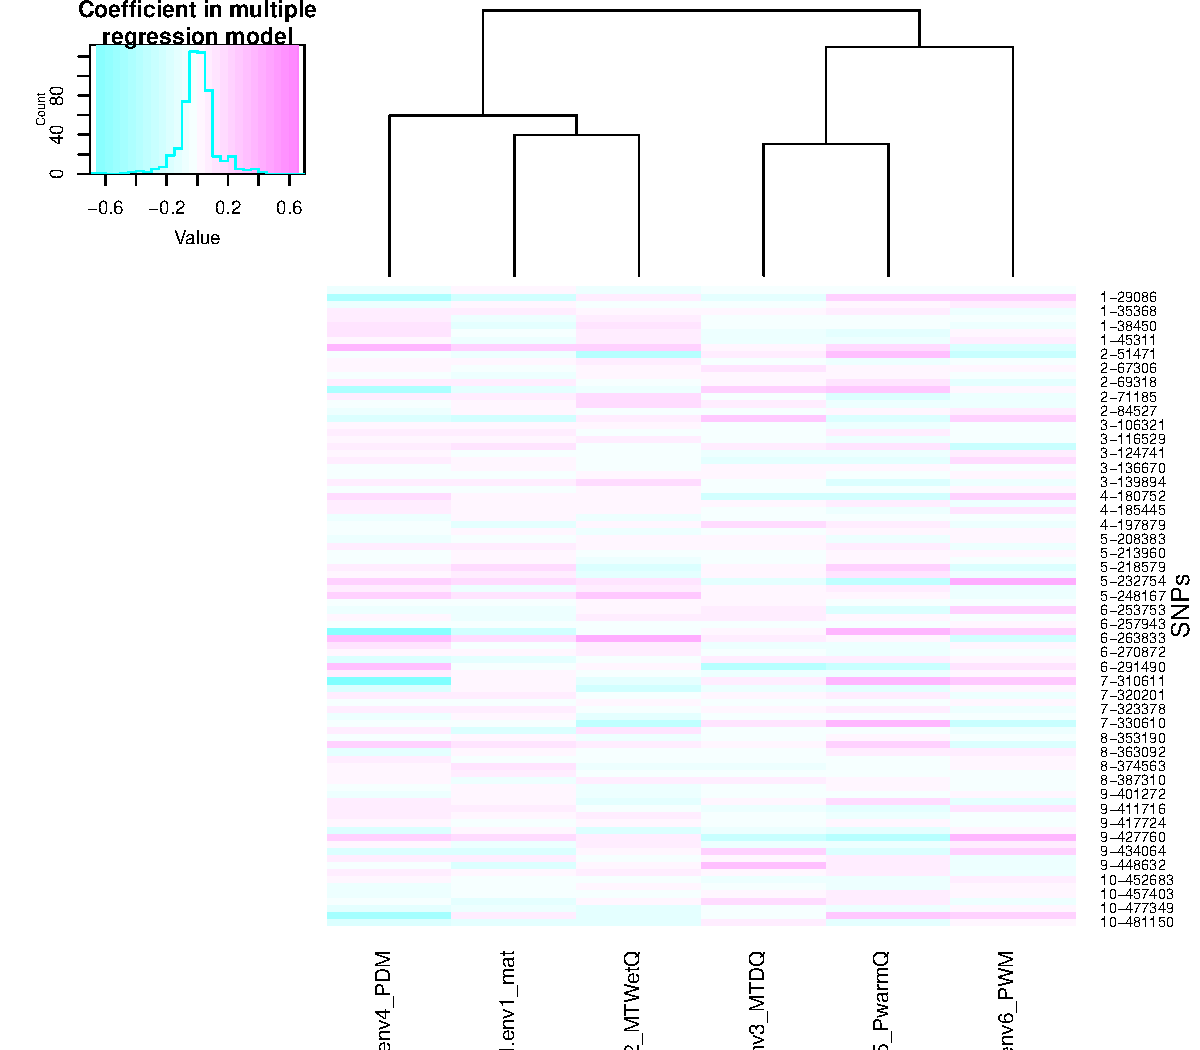
\includegraphics{RDAtraitPredictionTutorial_files/figure-latex/unnamed-chunk-7-1.pdf}

In the above heatmap, each row is a SNP. The SNPs are named according to
their linkage group (1 through 10) and cumulative position in the genome
(e.g.~9-448632 is on the 9th linkage group). Each linkage group was
50,000 bases long, so the cumulative position ranges from 1 to 500,000
over the 10 linkage groups. Each column in the heatmap is an
environment, which is an explanatory variable in the model.

The color of the heatmap cells for a SNP shows the coefficients in the
multiple regression model for each corresponding environment. In other
words, the colors show how environments are combined in a multiple
regression model to predict the patterns at that SNP on the landscape.

If we want to visualize clusters of SNPs that have similar coefficients
in the multiple regression model, we can allow for clustering in the
heatmap:

\begin{Shaded}
\begin{Highlighting}[]
\FunctionTok{heatmap.2}\NormalTok{(}\FunctionTok{t}\NormalTok{(Qr.coeff[,}\FunctionTok{which}\NormalTok{(muts}\SpecialCharTok{$}\NormalTok{causal)]),}
        \AttributeTok{scale=}\StringTok{"none"}\NormalTok{, }
        \AttributeTok{col =} \FunctionTok{cm.colors}\NormalTok{(}\FunctionTok{length}\NormalTok{(brks)}\SpecialCharTok{{-}}\DecValTok{1}\NormalTok{), }
        \AttributeTok{breaks=}\NormalTok{brks,}
        \AttributeTok{dendrogram =} \StringTok{"both"}\NormalTok{,}
        \AttributeTok{Rowv=}\ConstantTok{TRUE}\NormalTok{, }
        \AttributeTok{trace=}\StringTok{"none"}\NormalTok{,}
        \AttributeTok{key.title =} \StringTok{"Coefficient in multiple}\SpecialCharTok{\textbackslash{}n}\StringTok{regression model"}\NormalTok{,}
        \AttributeTok{ylab=}\StringTok{"SNPs"}\NormalTok{,}
        \AttributeTok{cexCol=}\DecValTok{1}\NormalTok{)}
\end{Highlighting}
\end{Shaded}

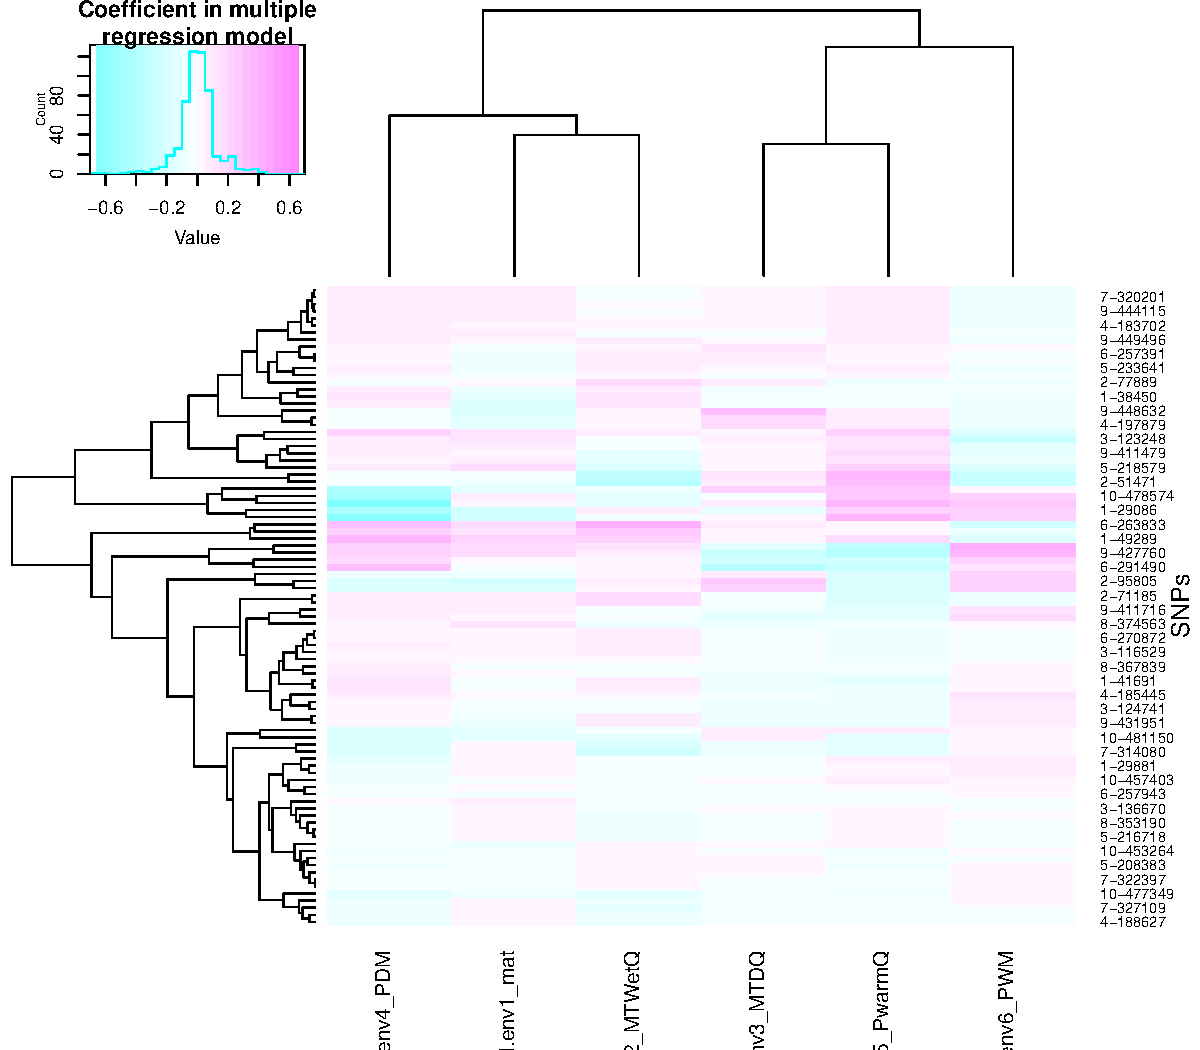
\includegraphics{RDAtraitPredictionTutorial_files/figure-latex/unnamed-chunk-8-1.pdf}

Here is the information about the session when the tutorial was built:

\begin{Shaded}
\begin{Highlighting}[]
\FunctionTok{sessionInfo}\NormalTok{()}
\end{Highlighting}
\end{Shaded}

\begin{verbatim}
## R version 4.2.2 (2022-10-31)
## Platform: aarch64-apple-darwin20 (64-bit)
## Running under: macOS Ventura 13.1
## 
## Matrix products: default
## BLAS:   /Library/Frameworks/R.framework/Versions/4.2-arm64/Resources/lib/libRblas.0.dylib
## LAPACK: /Library/Frameworks/R.framework/Versions/4.2-arm64/Resources/lib/libRlapack.dylib
## 
## locale:
## [1] en_US.UTF-8/en_US.UTF-8/en_US.UTF-8/C/en_US.UTF-8/en_US.UTF-8
## 
## attached base packages:
## [1] stats     graphics  grDevices utils     datasets  methods   base     
## 
## other attached packages:
## [1] gplots_3.1.3    lfmm_1.1        LEA_3.10.2      vegan_2.6-4    
## [5] lattice_0.20-45 permute_0.9-7  
## 
## loaded via a namespace (and not attached):
##  [1] Rcpp_1.0.10        rstudioapi_0.14    knitr_1.42         cluster_2.1.4     
##  [5] splines_4.2.2      MASS_7.3-58.2      rlang_1.0.6        fastmap_1.1.0     
##  [9] foreach_1.5.2      highr_0.10         caTools_1.18.2     tools_4.2.2       
## [13] parallel_4.2.2     grid_4.2.2         nlme_3.1-162       mgcv_1.8-41       
## [17] xfun_0.37          KernSmooth_2.23-20 cli_3.6.0          gtools_3.9.4      
## [21] htmltools_0.5.4    iterators_1.0.14   yaml_2.3.7         digest_0.6.31     
## [25] Matrix_1.5-3       bitops_1.0-7       codetools_0.2-19   evaluate_0.20     
## [29] rmarkdown_2.20     compiler_4.2.2
\end{verbatim}

\end{document}
